%  LaTeX support: latex@mdpi.com 
%  In case you need support, please attach all files that are necessary for compiling as well as the log file, and specify the details of your LaTeX setup (which operating system and LaTeX version / tools you are using).

%=================================================================
\documentclass[sustainability,article,submit,moreauthors,pdftex]{Definitions/mdpi} 

% If you would like to post an early version of this manuscript as a preprint, you may use preprint as the journal and change 'submit' to 'accept'. The document class line would be, e.g., \documentclass[preprints,article,accept,moreauthors,pdftex]{mdpi}. This is especially recommended for submission to arXiv, where line numbers should be removed before posting. For preprints.org, the editorial staff will make this change immediately prior to posting.

%--------------------
% Class Options:
%--------------------
%----------
% journal
%----------
% Choose between the following MDPI journals:
% acoustics, actuators, addictions, admsci, aerospace, agriculture, agriengineering, agronomy, algorithms, animals, antibiotics, antibodies, antioxidants, applsci, arts, asc, asi, atmosphere, atoms, axioms, batteries, bdcc, behavsci , beverages, bioengineering, biology, biomedicines, biomimetics, biomolecules, biosensors, brainsci , buildings, cancers, carbon , catalysts, cells, ceramics, challenges, chemengineering, chemistry, chemosensors, children, cleantechnol, climate, clockssleep, cmd, coatings, colloids, computation, computers, condensedmatter, cosmetics, cryptography, crystals, dairy, data, dentistry, designs , diagnostics, diseases, diversity, drones, econometrics, economies, education, ejihpe, electrochem, electronics, energies, entropy, environments, epigenomes, est, fermentation, fibers, fire, fishes, fluids, foods, forecasting, forests, fractalfract, futureinternet, futurephys, galaxies, games, gastrointestdisord, gels, genealogy, genes, geohazards, geosciences, geriatrics, hazardousmatters, healthcare, heritage, highthroughput, horticulturae, humanities, hydrology, ijerph, ijfs, ijgi, ijms, ijns, ijtpp, informatics, information, infrastructures, inorganics, insects, instruments, inventions, iot, j, jcdd, jcm, jcp, jcs, jdb, jfb, jfmk, jimaging, jintelligence, jlpea, jmmp, jmse, jnt, jof, joitmc, jpm, jrfm, jsan, land, languages, laws, life, literature, logistics, lubricants, machines, magnetochemistry, make, marinedrugs, materials, mathematics, mca, medicina, medicines, medsci, membranes, metabolites, metals, microarrays, micromachines, microorganisms, minerals, modelling, molbank, molecules, mps, mti, nanomaterials, ncrna, neuroglia, nitrogen, notspecified, nutrients, ohbm, optics, particles, pathogens, pharmaceuticals, pharmaceutics, pharmacy, philosophies, photonics, physics, plants, plasma, polymers, polysaccharides, preprints , proceedings, processes, proteomes, psych, publications, quantumrep, quaternary, qubs, reactions, recycling, religions, remotesensing, reports, resources, risks, robotics, safety, sci, scipharm, sensors, separations, sexes, signals, sinusitis, smartcities, sna, societies, socsci, soilsystems, sports, standards, stats, surfaces, surgeries, sustainability, symmetry, systems, technologies, test, toxics, toxins, tropicalmed, universe, urbansci, vaccines, vehicles, vetsci, vibration, viruses, vision, water, wem, wevj

%---------
% article
%---------
% The default type of manuscript is "article", but can be replaced by: 
% abstract, addendum, article, benchmark, book, bookreview, briefreport, casereport, changes, comment, commentary, communication, conceptpaper, conferenceproceedings, correction, conferencereport, expressionofconcern, extendedabstract, meetingreport, creative, datadescriptor, discussion, editorial, essay, erratum, hypothesis, interestingimages, letter, meetingreport, newbookreceived, obituary, opinion, projectreport, reply, retraction, review, perspective, protocol, shortnote, supfile, technicalnote, viewpoint
% supfile = supplementary materials

%----------
% submit
%----------
% The class option "submit" will be changed to "accept" by the Editorial Office when the paper is accepted. This will only make changes to the frontpage (e.g., the logo of the journal will get visible), the headings, and the copyright information. Also, line numbering will be removed. Journal info and pagination for accepted papers will also be assigned by the Editorial Office.

%------------------
% moreauthors
%------------------
% If there is only one author the class option oneauthor should be used. Otherwise use the class option moreauthors.

%---------
% pdftex
%---------
% The option pdftex is for use with pdfLaTeX. If eps figures are used, remove the option pdftex and use LaTeX and dvi2pdf.

%=================================================================
\firstpage{1} 
\makeatletter 
\setcounter{page}{\@firstpage} 
\makeatother
\pubvolume{xx}
\issuenum{1}
\articlenumber{5}
\pubyear{2019}
\copyrightyear{2019}
%\externaleditor{Academic Editor: name}
\history{Received: date; Accepted: date; Published: date}
%\updates{yes} % If there is an update available, un-comment this line

%% MDPI internal command: uncomment if new journal that already uses continuous page numbers 
%\continuouspages{yes}

%------------------------------------------------------------------
% The following line should be uncommented if the LaTeX file is uploaded to arXiv.org
%\pdfoutput=1

%=================================================================
% Add packages and commands here. The following packages are loaded in our class file: fontenc, calc, indentfirst, fancyhdr, graphicx, lastpage, ifthen, lineno, float, amsmath, setspace, enumitem, mathpazo, booktabs, titlesec, etoolbox, amsthm, hyphenat, natbib, hyperref, footmisc, geometry, caption, url, mdframed, tabto, soul, multirow, microtype, tikz

%=================================================================
%% Please use the following mathematics environments: Theorem, Lemma, Corollary, Proposition, Characterization, Property, Problem, Example, ExamplesandDefinitions, Hypothesis, Remark, Definition, Notation, Assumption
%% For proofs, please use the proof environment (the amsthm package is loaded by the MDPI class).

\graphicspath{ {./Figures/} }

%=================================================================
% Full title of the paper (Capitalized)
\Title{Exploring the Socioeconomic Co-benefits of Global Environment Facility Projects in Uganda using a Quasi-experimental Geospatial Interpolation (QGI) Approach}

% Author Orchid ID: enter ID or remove command
\newcommand{\orcidauthorA}{0000-0001-5356-4676} % Add \orcidA{} behind the author's name
%\newcommand{\orcidauthorB}{0000-0000-000-000X} % Add \orcidB{} behind the author's name

% Authors, for the paper (add full first names)
\Author{Daniel Runfola $^{1,2,*}$\orcidA{}, Geeta Batra $^{3}$, Anupam Anand $^{3}$, Audrey Way$^{1,2}$, and Seth Goodman $^{1}$}

% Authors, for metadata in PDF
\AuthorNames{Daniel Runfola, Geeta Baatra, Anupam Anand and Seth Goodman}

% Affiliations / Addresses (Add [1] after \address if there is only one affiliation.)
\address{%
$^{1}$ \quad Department of Applied Science, William \& Mary\\
$^{2}$ \quad Geospatial Evaluation and Observation Lab, William \& Mary \\
$^{3}$ \quad Independent Evaluation Office, Global Environment Facility}

% Contact information of the corresponding author
\corres{Correspondence: danr@wm.edu; Tel.: +1-757-221-1970; Web: geolab.wm.edu}

% Current address and/or shared authorship
% The commands \thirdnote{} till \eighthnote{} are available for further notes

%\simplesumm{} % Simple summary

%\conference{} % An extended version of a conference paper

% Abstract (Do not insert blank lines, i.e. \\) 
\abstract{Between 2002 and 2014, the Global Environment Facility mobilized USD \$10.47 billion in funds to enable developing and transitioning countries to meet the objectives of international environmental conventions and agreements. While multiple studies and reports have sought to examine the environmental impact of these funds, relatively little work has examined the potential for socioeconomic co-benefits. Leveraging a novel database on the geographic location of GEF project interventions in Uganda, this paper explores the impact of GEF projects on household assets in Uganda.  It employs a new methodological approach, Quasi-experimental Geospatial Interpolation (QGI), which seeks to overcome many of the core biases and limitations of previous implementations of causal matching studies leveraging geospatial information.  Findings suggest that Sustainable Forest Management (SFM) GEF projects with initial implementation dates prior to 2009 in Uganda had a positive, statistically significant impact of approximately USD \$184.81 on the change in total household assets between 2009 and 2011.  Leveraging QGI, we identify that (1) this effect was statistically significant at distances between 2 and 7 kilometers away from GEF projects, (2) the effect was positive but not statistically significant at distances less than 2km, and (3) there was insufficient evidence to establish the impact of projects beyond a distance of approximately 7km.}

% Keywords
\keyword{Cobenefits, Sustainable Development, Causal Methods, Geospatial Impact Evaluation, Quasi-experimental design, Interpolation, GIS, Remote Sensing}

% The fields PACS, MSC, and JEL may be left empty or commented out if not applicable
%\PACS{J0101}
%\MSC{}
%\JEL{}

%\setcounter{secnumdepth}{4}
%%%%%%%%%%%%%%%%%%%%%%%%%%%%%%%%%%%%%%%%%%
\begin{document}
%%%%%%%%%%%%%%%%%%%%%%%%%%%%%%%%%%%%%%%%%%

%%%%%%%%%%%%%%%%%%%%%%%%%%%%%%%%%%%%%%%%%%

%%% Citing a journal paper \cite{ref-journal}. And now citing a book reference \cite{ref-book}. 

\section{Introduction}
Since the Rio Earth Summit in 1992, the Global Environment Facility (GEF) has been one of the largest actors in the environmental sector, with a portfolio of activities worth over \$24 billion USD.  With the explicit goal of supporting international environmental conventions and agreements, a number of these projects have been subjected to intense evaluation by the GEF Independent Evaluation Office (IEO) to assess their effectiveness in terms of environmental outcomes. However, relatively little research has been conducted to examine the socioeconomic co-benefits that may accrue due to environmental interventions.  This is reflective of a broader shortage of impact evaluations of development projects, as the primary environmental impacts of development projects and programs are rarely assessed and quantified conclusively \cite{AlpizarTheRCTs}. Recognizing this gap in the literature, and leveraging a unique spatial dataset and methodology, this paper explores the research question:  \textit{What was the impact of GEF Sustainable Forest Management projects on household income in Uganda between 2009 and 2011}.  
\par
To examine this question, we introduce a new method called Quasi-experimental Geospatial Interpolation (QGI).  QGI is a matching-based approach to causal inference using historic, spatial data on the location of interventions of interest (i.e., a GEF project).  These spatial locations at which a GEF intervention occurred are contrasted to spatial locations at which an intervention did not occur, but were otherwise as similar as possible, following increasingly common spatial propensity score matching approaches \cite{Runfola2017wb, MalteUitto2018ImprovingAnalysis}.  QGI mitigates two core shortfalls of existing spatial propensity score matching methods. First, it explicitly provides a measurement of the relationship between distance and impact effect, allowing for analyses of the distance(s) away from an intervention at which effects are no longer detectable.  Second, it provides a formalized approach to identifying spatial matches that ensure key statistical principals are not violated (specifically focusing on the Stable Unit Treatment Value Assumption [SUTVA]), minimizing the chance of model selection bias through "p-score hacking" or other similar techniques.
\par
The paper is structured as follows.  First, we provide a background literature review on environmental co-benefits as they relate to GEF projects in section \ref{sub:cobenefits}.  Second, in \ref{sub:qm} we explore the literature on spatial propensity score matching, and summarize the gaps in that literature.  In section \ref{sub:data} we present the data used for this analysis, and section \ref{sub:methods} introduces the Quasi-experimental Geospatial Interpolation approach.  Sections \ref{results} and \ref{conclusion} provide our results and conclusions, respectively.


\subsection{Literature Review - Environmental Co-benefits}\label{sub:cobenefits}
We have limited and inconsistent evidence on the environmental co-benefits of poverty programs, and similarly on the socio-economic impacts of environmental interventions \cite{AlpizarTheRCTs, Naidoo2019EvaluatingWorld, McKinnon2016WhatCountries}. This gap is a reflection of widespread uncertainty about the impact of conservation and development interventions. Studies that have tried to address this have various limitations, including methodology and data, and their varying temporal and spatial scales make it a challenge to draw general conclusions \cite{Naidoo2019EvaluatingWorld, AlpizarTheRCTs}. Recently, a small number of observational studies have attempted to quantify the causal effects of environmental programs on socio-economic outcomes (e.g., \cite{Oldekop2019ReductionsNepal, Naidoo2019EvaluatingWorld, Ferraro2014QuantifyingInfrastructure}; a smaller number have attempted to quantify the causal effects of poverty programs on the environment (e.g., Alix-Garcia et al. 2013). 
\par
In 2019, Alpizar and Ferraro \cite{AlpizarTheRCTs} highlighted the potential of randomized control trials (RCTs) to unravel the processes between poverty reduction activities and actions to protect the environment. The study highlighted the absence of robust experimental design such as RCTs in environmental programs - while at the same time, RCTs involving anti-poverty interventions rarely assess their environmental effects.  Other innovative study methods to examine environmental co-benefits include the use of socio-ecological approaches and complexity theory to measure all the outcomes that are influenced/associated by the interventions and not merely measuring the components that are mentioned in the project or program documents. However, many of these approaches are underdeveloped at this stage.  Given the gaps discussed above, contributing to this area of research in the context of the GEF will be essential to inform further how targeted investments in the environment can also contribute to poverty reduction and human development in addition to generating environmental benefits.

\subsection{Literature Review - Quasi-experimental Models with Spatial Data}\label{sub:qm}
Recent literature has examined many of the unique challenges of applying causal models to spatially explicit interventions. To provide a brief introduction, estimation for the purpose of causal attribution generally seeks to fit a model of a form similar to:
\begin{equation}\label{basic_theta}
y_{i} = \beta0 + \theta * T_{i} + \beta_{j} * X_{i,j} 
\end{equation} 
where $y_{i}$ is the outcome of interest (i.e., income), $\theta$ is the intervention (or treatment) effect on the outcome of interest for which an accurate estimate is desired, $T_{i}$ represents a binary indication of if unit of observation $i$ received a given intervention, $\beta_{j}$ represent parameters we seek to fit to control for potential effects from sources other than the intervention $j$, and $X_{i,j}$ represents the value for unit of observation i for each control variable $j$.  The most common approach to estimating $\theta$ is to construct a sample set in which all units that received an intervention ($T=1$) are matched with units that did not receive an intervention ($T=0$), where matches are conducted to minimize differences along relevant dimensions (``twins").  Observations which are not a part of an optimally paired twin in the dataset are either removed (in one-to-one matching) or weighted (in many-to-one matching).  This sample set is then used to estimate equation \eqref{basic_theta}. 
\par
When using historical data - such as the data on past GEF projects used in this paper - we must search across all available observations to establish if sufficient information exists to conduct an analysis with matched observations.  Approaches leveraging historic data (rather than collecting new data in controlled settings) are broadly referred to as quasi-observational, with a goal of minimizing the impact of non-random allocation of interventions on estimates of $\theta$.  In the most popular framework for quasi-observational designs, the Rubin causal model, matching strategies which pair control and treatment units are expanded to attempt to minimize differences explicitly along dimensions that were not random in respect to treatment assignment - i.e., control and treatment cases are preferentially matched along dimensions treatment assignment occurred.  
\par
As matching strategies are increasingly performed using spatial data, researchers have begun to consider the unique challenges this brings.  These include:
\begin{enumerate}
    \item The spatial spillover of intervention effect from recipient regions to neighboring regions \cite{Runfola2017wb, Buchanan2016TheImportance}.
    \item The spatial imprecision of measurement in where interventions are implemented \cite{Marty2019AssessingImprecision}.
    \item The robustness of selecting different distance bands to distinguish between areas determined to be ``treated'' as contrasted to ``untreated'' \cite{BunteNaturalLiberia}.
\end{enumerate}
This paper provides a generic approach for engaging with challenges related to the first and third of these methodological challenges - spatial spillover and robustness of distance band selection.  We refer readers to \cite{Marty2019AssessingImprecision} for an inter-operable solution to the second enumerated challenge above.  The challenge of spatial spillover is well summarized in \cite{Buchanan2016TheImportance} - specifically, the need to ensure that the units defined as "control" units (i.e., those that did not receive intervention) did not in any way benefit from the treatment.  In a spatial context, this is a common challenge - i.e., if a village is a beneficiary of a sustainable farming training program, individuals from neighboring villages may travel to attend, or information from the program may naturally diffuse along social networks.\footnote{This is also a challenge among treated units - i.e., a treatment effect may compound if more neighboring units are treated.  The method presented here does not explicitly estimate this compounding effect, but such effects would be included in the overall treatment effect estimate (see \cite{Corrado2012} for a complete conversation of the challenges of SUTVA with spatial data).}
\par
The challenge of selecting distance bands to distinguish between areas to be defined as ``treated'' or ``untreated'' is increasingly evident in the literature (see, for example, \cite{BunteNaturalLiberia, Buchanan2016TheImportance}).  This challenge relates to the unknown nature of how interventions will diffuse over geographic space - i.e., if an animal clinic might benefit farmers within 10 or 50 kilometers.  Because this distance threshold is generally unknown, researchers are left to arbitrarily determine a threshold at which they anticipate no effect would be reasonable to expect; locations beyond this threshold are defined as "control" units.  Arbitrarily choosing this distance can result in an increased likelihood of "p-score hacking", or selecting for distances at which a desired effect is identified; varying this distance can result in bias due to the fact that a single unit can be defined as a "treated" unit in one analysis, and a "control" in another.  We discuss how QGI engages and mitigates these challenges in section \ref{sub:methods}.

\section{Data and Methods}
\subsection{Data}\label{sub:data}
This paper leverages a novel dataset of Global Environment Facility Sustainable Forest Management projects, represented by thousands of spatial boundaries defining areas of intervention. This analysis relies on a subset of 33 project locations for which exact geographic boundaries are known\footnote{As noted in the introduction, this paper does not engage with questions of spatial imprecision for projects for which exact coordinates are not known; we refer readers to \cite{Marty2019AssessingImprecision} for solutions to that class of problem.}, which can be seen outlined in red in figure \ref{fig:data}. Criteria for selection included projects which had direct implementations (i.e., activities that would impact the geographic region of intervention), intersection with Uganda, and project implementation dates before our baseline period of 2009.  Projects include both small-scale projects implemented solely within Uganda, and regional-scale initiatives that were also inclusive of other projects within the region.  
\par
In addition to information on the geographic location of GEF SFM projects, data from the World Bank Living Standards Measurement Survey was used to estimate the outcome measure in this study - household assets.  Collected in 2009 and 2011 within Uganda, the LSMS provides geographic latitude and longitude information on where household clusters were surveyed, accurate to within 5 kilometers.  In both surveys, an identical question was asked which is used in this analysis - "What is the total estimated value of all the assets owned by your household?".  In 2009, the LSMS surveyed 2,960 households with an instrument that asked these questions; of these households, 2,926 provided a response to this information along with geographic location information.  In 2011, the LSMS surveyed 2,497 households, of which 2,316 households provided the same information.  The locations of these surveys can be seen in figure \ref{fig:data}.
\par
Finally, a set of geospatial covariates were retrieved and integrated into a standardized grid with a resolution of 10 kilometers following the approach outlined in \cite{goodman2019}; a full list of ancillary covariates is included in table \ref{table:data}.  The data collected from LSMS was aggregated to each cell to generate annual average measurements of household assets, and the distance between each cell and GEF SFM project was calculated. Ultimately, this resulted in a final dataset in which each row was representative of a 10 square kilometer region across Uganda (as shown in figure \ref{fig:data}), with each row containing measurements from the data sources in table \ref{table:data}. Yearly measurements were derived where feasible, with average, max, and minimum yearly values being retrieved and saved.  In temporally invariant cases such as roads, the distance to the nearest observation was calculated and assumed to be similar across the time periods surveyed (2009 and 2011).


\begin{figure}[ht]
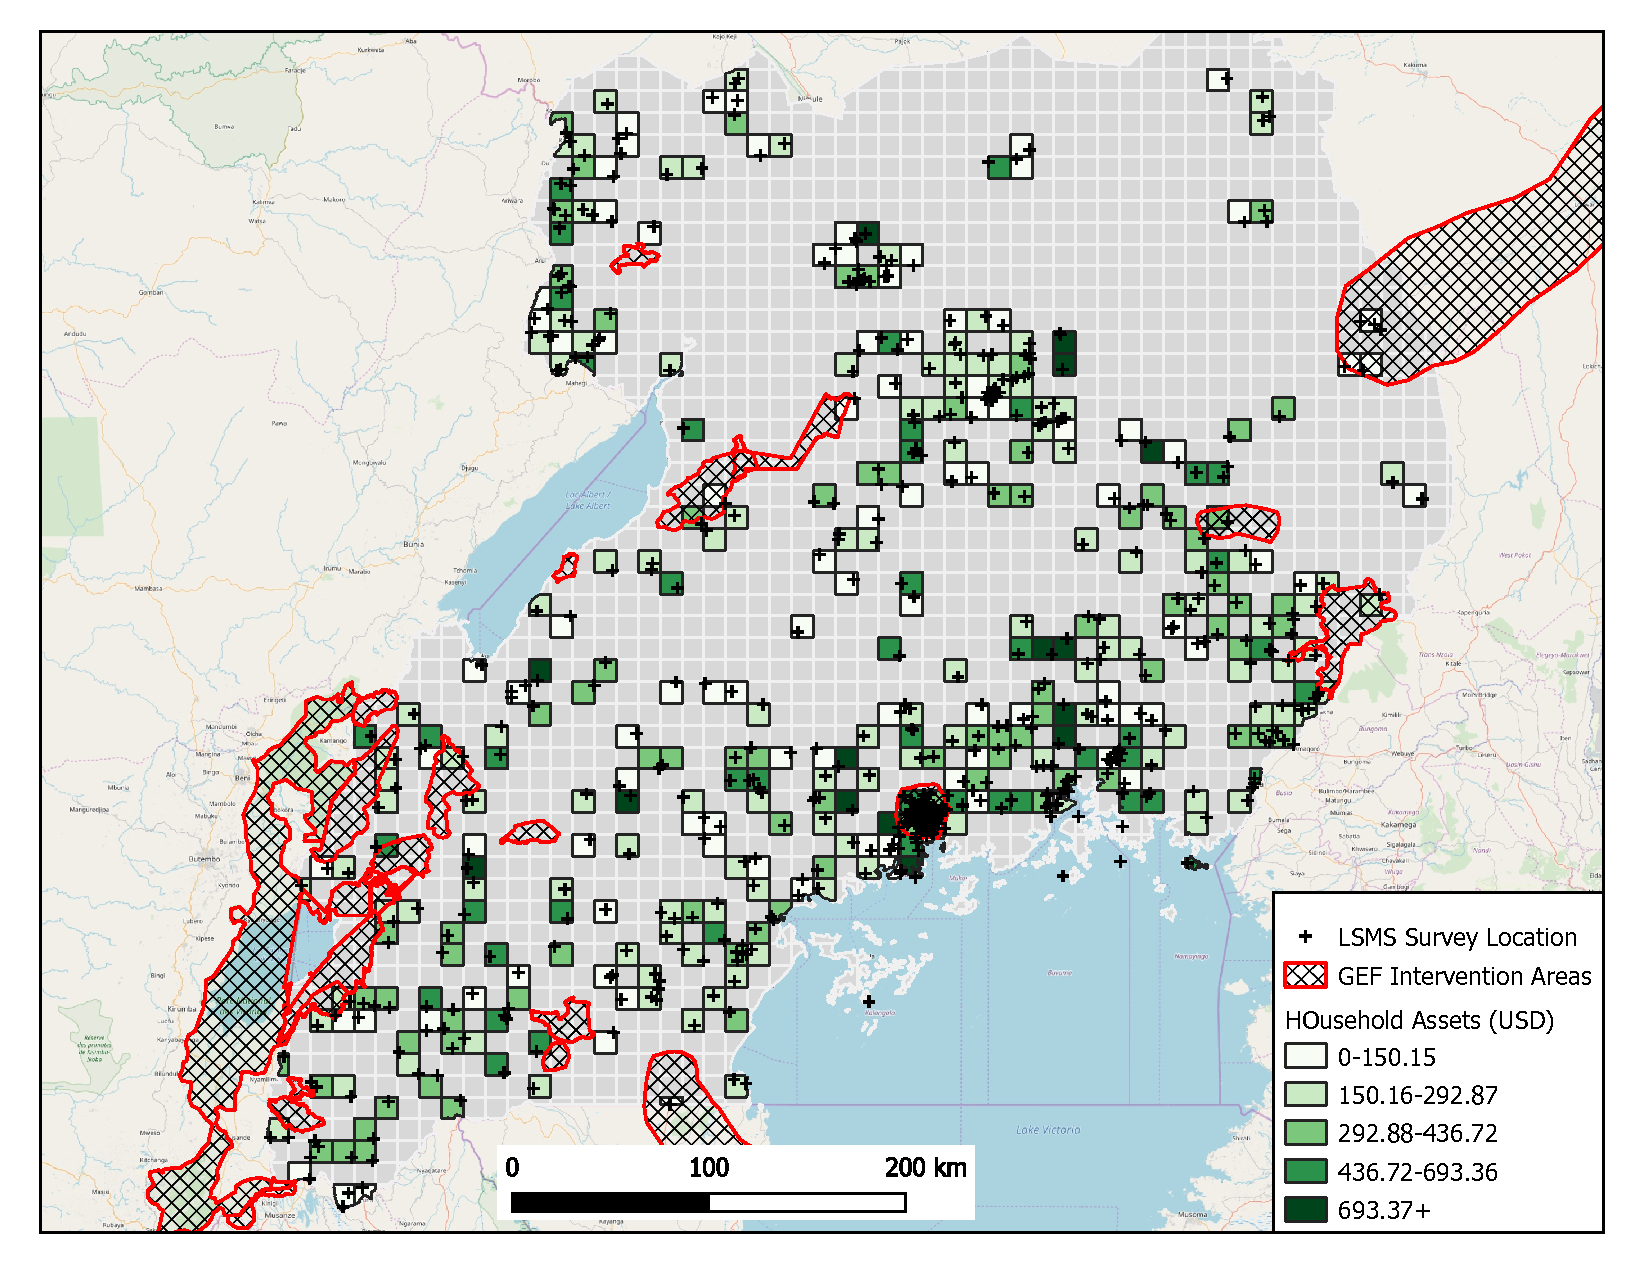
\includegraphics[width=\textwidth]{Figures/final_figure1.pdf}
\caption{Data used in this analysis. Grey areas indicate areas where no LSMS data was available, hashed areas with a red boundary indicate GEF project areas and green areas indicate areas where LSMS data was available. White or light green cells represent households with fewer assets in USD than darker green cells.}
\label{fig:data}
\end{figure}


\begin{table}[H]
\caption{Ancillary data used in this analysis.}
%% \tablesize{} %% You can specify the fontsize here, e.g., \tablesize{\footnotesize}. If commented out \small will be used.
\begin{tabular}{ccc}
\toprule
\textbf{Feature}	& \textbf{Source}	& \textbf{Resolution}\\
\midrule
Nighttime Lights&Defense Meteorological Satellite Program (DMSP-OLS) \cite{dmsp}			& 1km\\
&Visible Infrared Imaging Radiometer Suite (VIIRS) \cite{viirs} & 250m\\
Road Networks & Global Roads Open Access Data Set (gRoads) \cite{groadsv1} & 1km\\
Global Administrative Zones & geoBoundaries Administrative Zones\cite{geoboundaries}  & Variable \\
Protected Areas & World Database of Protected Areas (WDPA) \cite{wdpa} & Variable\\
Population & Gridded Population of the World (GPW) \cite{gpwv3count, gpwv4count} & 1km\\
Topology & Shuttle Radar Topography Mission (SRTM) \cite{nasasrtm}&500m\\
Air Temperature&University of Delaware \cite{udeltemp2014}&50km\\
Precipitation&University of Delaware\cite{udelprecip2014}&50km\\
Land Cover&European Space Agency\cite{esaland}&300m\\
Land Surface Temperature&MODIS\cite{modis}&1km\\
NDVI & NASA Long Term Data Record (LTRD)\cite{ltdr}&1km\\

\bottomrule
\label{table:data}
\end{tabular}
\end{table}

\subsection{Methods}\label{sub:methods}
This paper introduces a new method for the estimation of causal impacts of an intervention using spatial data, Quasi-experimental Geospatial Interpolation (QGI).  QGI builds on the geospatial matching methods noted in the literature review by providing diagnostics to examine the robustness of findings when the region an intervention might impact is not known.  We specifically seek a solution to the problem that a distance selected to demarcate the difference between "control" and "treatment" must be selected to build treatment and control groups, but frequently the correct distance is unknown (see, for example, figure \ref{fig:bands}).  Not only does this have implications for examining model robustness, but also for studies that seek to identify the spatial distances at which effects may (or may not) be detectable.

\begin{figure}[!ht]
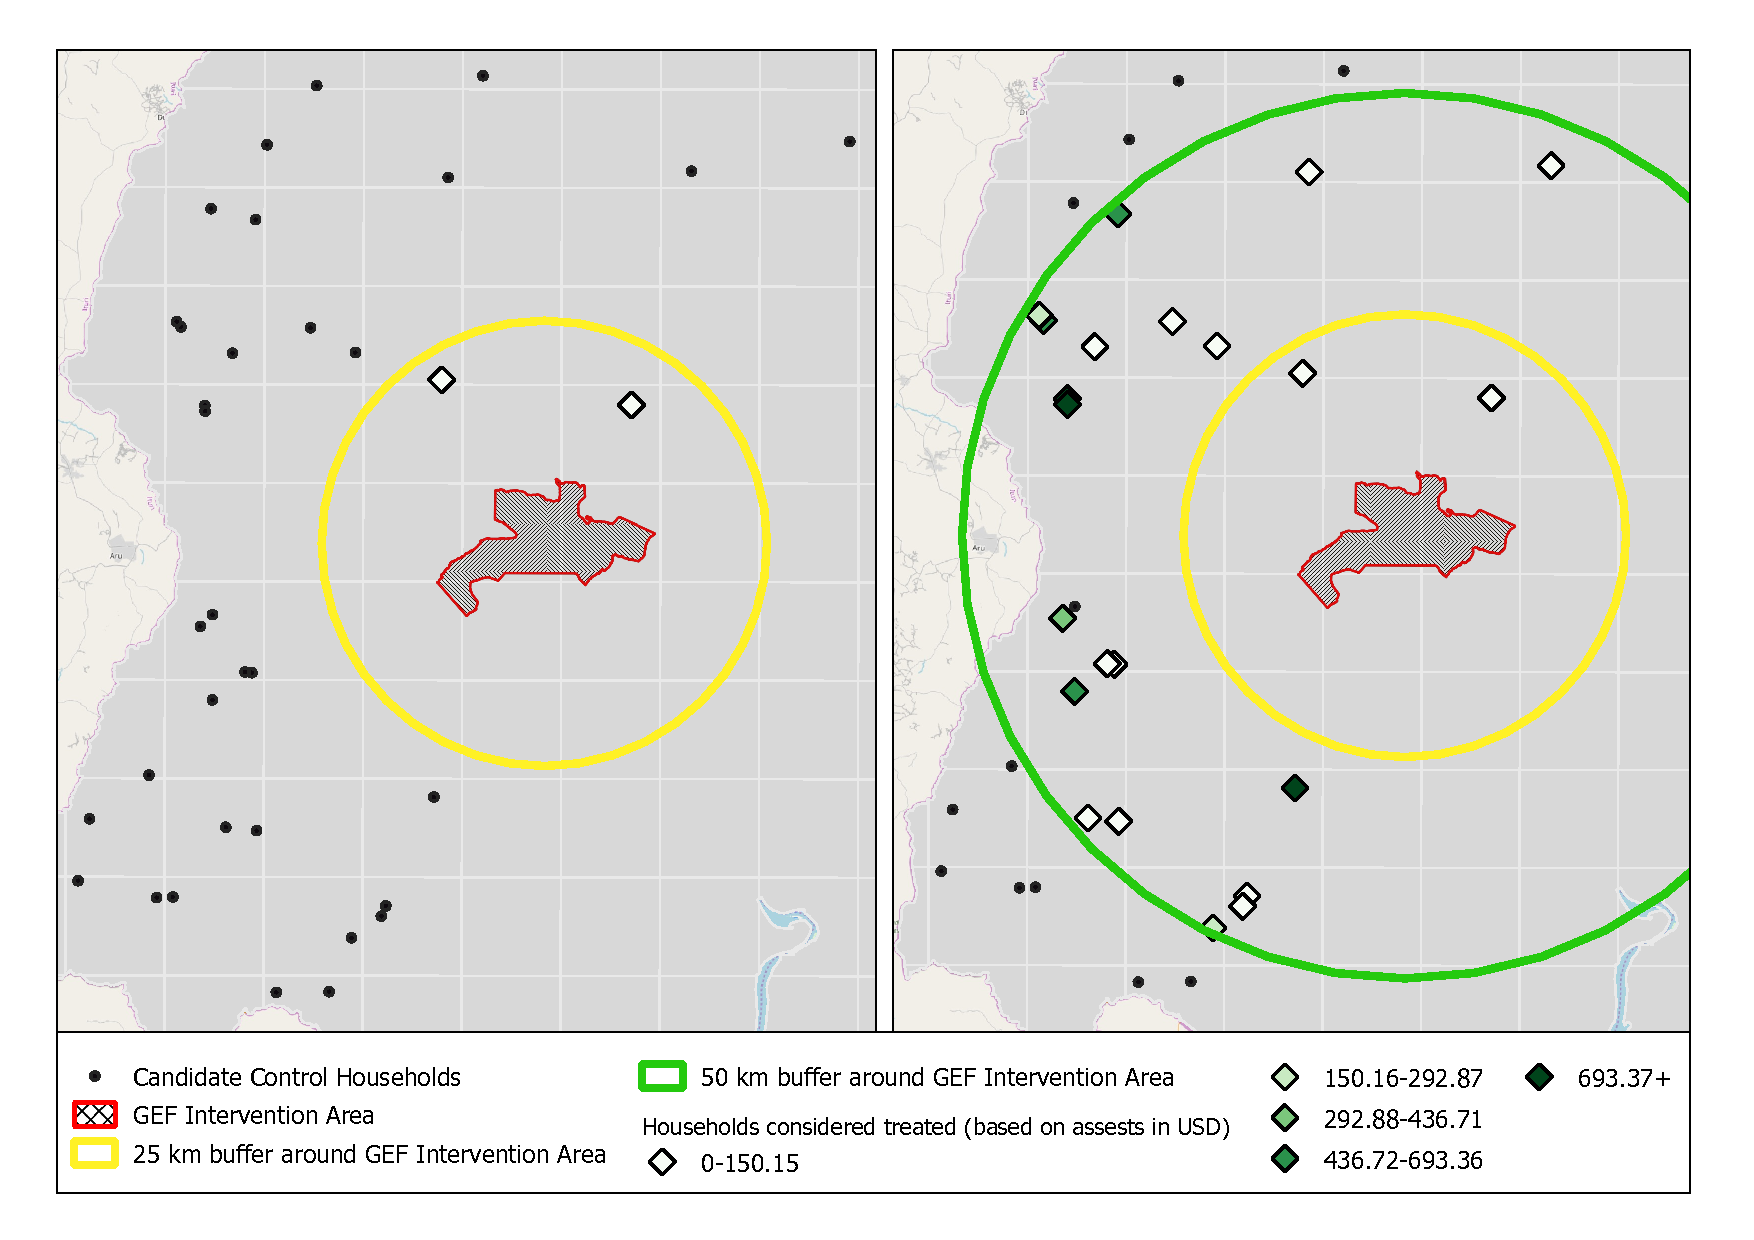
\includegraphics[width=\textwidth]{Figures/final_figure2.pdf}
\caption{Two alternative scenarios for an impact evaluation in which the effect of a GEF project (outlined in red) is estimated.  In the left case, a distance of 25 kilometers is chosen for a buffer which determines the units that are treated (denoted by diamonds).  In the right case, a 50km buffer is chosen.  As can be seen in this figure, many of the units of observation that would be considered "control" cases in the left figure would become "treated" cases in the right figure.}
\label{fig:bands}
\end{figure}

QGI engages with this challenge by seeking to explicitly model the distance-decay function of the treatment estimate ($\theta$ in equation \eqref{basic_theta}) through an iterative approach of changing the distance thresholds at which controls and treatments are demarcated (similar to the approach adopted by kriging-based spatial interpolation).  It follows a three step process in which:
\begin{enumerate}
    \item Two hyperparameters are chosen:
    \begin{enumerate}
        \item The maximum distance ($\delta$) for which a treatment effect will be constructed.
        \item The number of distance bands $\kappa$, with the geographic distance for each band denoted by $\kappa_{i}$.
    \end{enumerate}
    \item For each distance $\kappa_{i}$:
    \begin{enumerate}
        \item All units of observation that are geographically closer to an intervention than the specified $\kappa_{i}$ are considered as "treated".
        \item These units are matched with eligible control units that have a minimum distance away from an intervention site of $\delta$.
        \item The quality of the matches ($\phi_{i}$) is calculated and recorded.
        \item A regression model, similar to that in eq. \eqref{basic_theta}, is estimated;  both $\theta_{i}$ and the standard deviation $\sigma_{i}$ are recorded.
    \end{enumerate}
    \item After $\theta$ is recorded for all distance bands $i$, the relationship between distance and $\theta$ is estimated using a model of the users choice - i.e., spherical or polynomial, with a weighting approach in which distance bands with better match qualities ($\phi_{i}$) are given more weight.  This is repeated for the standard deviation of the estimates ($\sigma$).
\end{enumerate}

\begin{figure}[!ht]
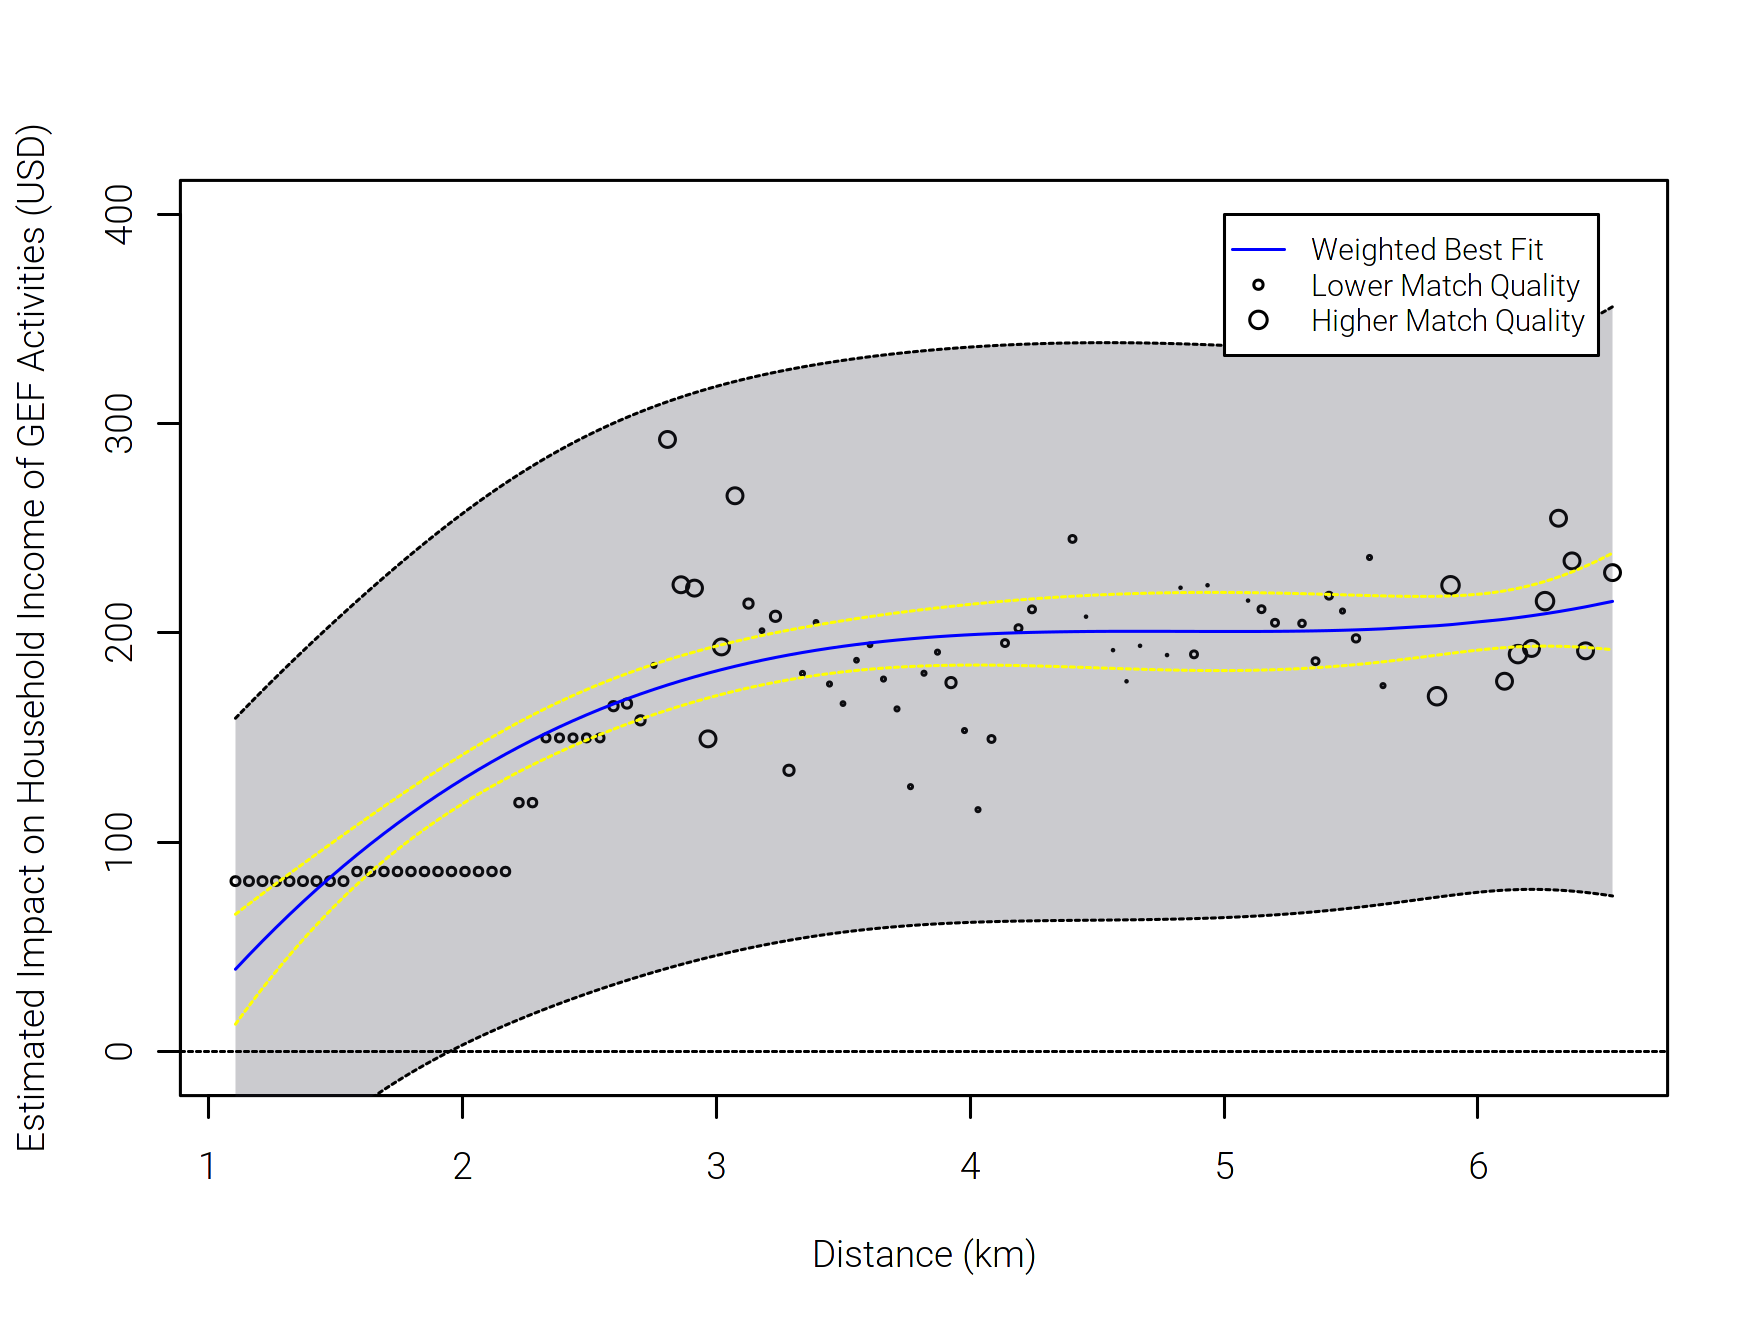
\includegraphics[width=\textwidth]{Figures/GEF_distanceDecay.png}
\caption{Estimated effect of GEF SFM interventions in Uganda, based on improvements in household assets.  The grey region indicates the modeled standard errors for each distance; the yellow lines denote uncertainty due to the spatial interpolation approach.}
\label{fig:GEF}
\end{figure}

Following this approach, the relationship between distance, standard errors and estimated treatment effect can be visualized as illustrated in figure \ref{fig:GEF}. The full procedure is detailed below in section \ref{results}, using the case study of Uganda as an illustrative example.  


%%%%%%%%%%%%%%%%%%%%%%%%%%%%%%%%%%%%%%%%%%
\section{Results}\label{results}
This section introduces QGI using an illustrative case study in Uganda; the subsections here are reflective of each of the steps outlined in section \ref{sub:methods}. 
\subsection{Hyperparameter Selection}
Two hyperparameters must be selected to implement QGI - $\delta$, or the maximum distance for which an effect will be estimated, and $\kappa$, or the number of distance bands for which effects will be estimated (i.e., the resolution of the estimation).  For this analysis, an upper distance bound of $\delta \approx 50km$ was selected as a theoretical approximation of the maximum distance for which an effect could be detected \footnote{As the reader will see in later sections, the resultant estimate is - in this case - insensitive to this choice, as the maximum distance for which the data support conclusions is approximately 7km.}.  $\kappa$ was selected according to available computation, with 30 iterations being performed on each of 16 compute cores available (for a total of $\kappa = 480$)\footnote{Initial exploration suggests that - for reasonably smooth surfaces - results are robust across multiple $\kappa$ selections.}.  

\subsection{Model Estimation for Distances $\kappa_{i}$}
Within Uganda, we seek to contrast households surveyed by LSMS proximate to GEF projects to those that are not proximate.  The goal of this contrast is to estimate the effect of GEF projects on household assets at these households.  This subsection describes the iterative model fitting procedure in which we contrast "close" households to "far" households, with the distance band defining "close" ($kappa_{i}$) increasing at each step until the maximum step $\delta$ is reached.
\par
As an illustrative example, we will explore $kappa_{41}$; this iteration is chosen as the distance $kappa_{41}$ is approximately equal to 5km.  Given the above $\delta$ of approximately 50km, the goal of this model iteration is to contrast all LSMS households that fall within 5km of a GEF project implementation to LSMS households that fall at least 50km away from a GEF project implementation.
\par
To accomplish this contrast, a series of three equations are estimated.  First, we model the likelihood that any unit might have received an intervention - referred to as a propensity score:
\begin{equation}
    T_{j} = \beta_{0} + \beta_{k} * X_{k,j}
\end{equation}

where $T_{j}$ is a binary value indicating if LSMS household location $j$ is within 5km of a GEF project; $\beta_0$ is an intercept, $\beta_{k}$ is a fitted parameter value for covariate k, and $X_{k,j}$ is covariate $k$'s value for LSMS household location $j$.  Each covariate listed in table \ref{table:data} is included.  An optimal parameterization of this model is identified through a logistic regression least squares approach, and the resultant propensity score predicted for every unit of observation $j$ are saved as $P_{j}$.  For every treated unit $T_{j} = 1$, the single control unit $T_{j} = 0$ with the most similar propensity score is identified and saved; a final dataset is then constructed that only contains these matches (unmatched cases of $T_{j} = 0$ are discarded).\footnote{We do not go into detail on the theoretical underpinnings of propensity score matching for causal inference in this paper; rather, we direct readers to \cite{ZhaoQuantifyingProjects}.}  Finally, the quality of matches for distance band $kappa_{i}$ are calculated by taking the absolute value of the difference between the average propensity score for treated and untreated cases:
\begin{equation}
    \left | \left (  \frac{P_{j}* T_{j}}{N} \right ) - \left (  \frac{P_{j}* \left|T_{j}-1\right |}{N} \right )  \right |
\end{equation}
\par
After matching, constructing a new dataset which only includes matched cases, and recording the overall match quality $\phi$, a linear regression model is fit:
\begin{equation}
    Household Assets_{j} = \beta_{0} + \theta * T_{j} + \beta_{k} * X_{k,j}
\end{equation}
in which the ultimate goal is to estimate $\theta$ with a high degree of accuracy. In this specific example, $\theta_{i}$ can be interpreted for $\kappa_{41}$ as the effect a GEF project has on household assets if a GEF project is located within approximately 5km.  Once this value is estimated, the standard error of the estimates ($\sigma_{i}$) is also recorded.  In the case of $i = 41$, $\theta_{41} = 209.41$ and $\sigma_{41} = 119.25$.  This process is repeated for every distance value $\kappa$, for a total of (in this case) 480 estimates of $\theta$ and $\sigma$.


 
\subsection{Estimating a Spatial Model for $\theta$ and $\sigma$}
With all 480 estimates of $\theta$ and $\sigma$, we seek to estimate the relationship between distance away from intervention and effectiveness.  While many methods for establishing the relationship between distance and an outcome of interest can be chosen, here we implement a weighted third order polynomial.  To fit this spatial model, first for each of our 480 iterations $i$ we drop any cases that did not have sufficient matches to fit a model estimate, or did not have at least a certain threshold of match quality (in this case, a difference of 0.1); once this dropping is done we calculate a weight for remaining cases based on the recorded $\phi_{i}$:
\begin{equation}
W_{i} = 1 - \left ( \frac{\phi_{i} - min(\phi)}{max(\phi) - min(\phi)}  \right )     
\end{equation}
this weighting approach gives the highest weight to the best relative match, and the least weight to the worst relative match.  At this stage, we have all data visualized in figure \ref{fig:exNoTrend}.  We use this information to estimate a 3rd order polynomial trend relating distance ($\kappa_{i}$) to the estimated treatment effect ($\theta_{i}$), adjusting the loss function from ordinary least squares to account for the weights provided be $\phi_{i}$:
\begin{equation}
\sum \phi_{i}*(\hat{\theta_{i}} - \theta_{i})^2
\end{equation}
By repeating this process for the standard errors recorded in each model iteration ($\sigma_{i}$), we can establish a predicted confidence interval around the polynomial trend line. By adding to the model standard errors the standard errors of the polynomial fit itself, we get a final envelope of possible errors for any given distance.  In the final figure, figure \ref{fig:GEF}, the blue line indicates the 3rd order polynomial trend relating $\theta$ and distance; the area bracketed by yellow lines indicates the standard errors attributable to uncertainty regarding the estimate of this trend.  The remainder of the grey region indicates standard errors attributable to the estimate of $\theta$ at each iteration $i$.  Of note is that lack of estimates beyond approximately 7km - this is due to insufficient matches of high enough quality to generate estimates beyond this point (i.e., the dropping procedure outlined earlier in this section).

\begin{figure}[!ht]
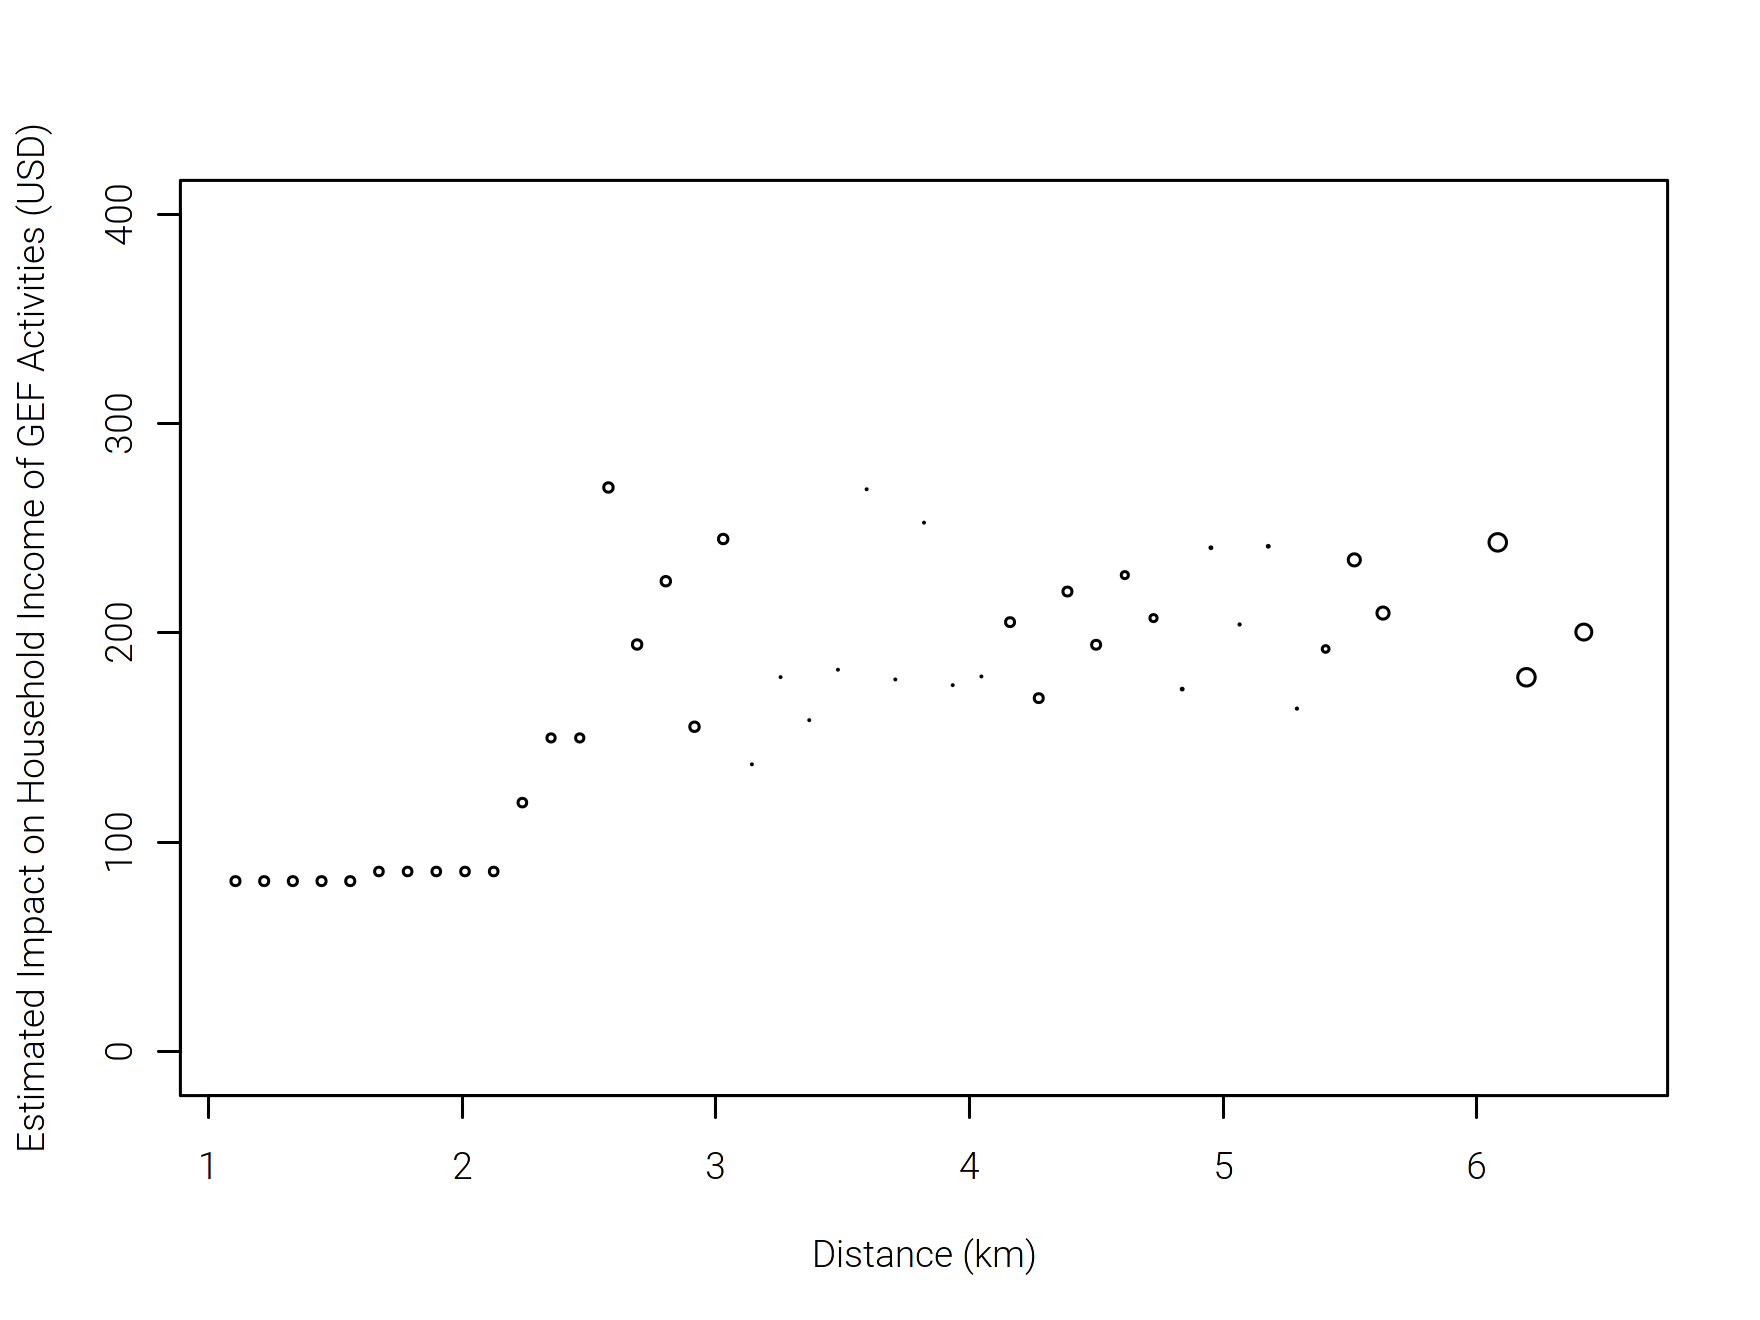
\includegraphics[width=\textwidth]{Figures/only_matches.png}
\caption{Matched propensity models estimating $\theta$ at difference distances.  Each dot represents a single iteration $i$, with the y-axis value indicating the estimated $\theta_{i}$, x-axis the distance $\kappa_{i}$, and the size of each point the relative weight $\phi_{i}$.}
\label{fig:exNoTrend}
\end{figure}

\section{Discussion \& Conclusions}\label{conclusion}
This paper sought to identify the relationship between the siting of GEF Sustainable Forest Management projects and changes in household assets in households proximate to those locations. By applying Quasi-experimental Geospatial Interpolation (QGI), we found robust and consistent evidence that the GEF had a positive impact on local household assets, to the order of approximately 184 USD between 2009 and 2011 (the survey years; figure \ref{fig:GEF}).  While all distances estimated in this study suggested a positive impact, distances greater than 2km illustrated statistically significant positive impacts.  Insufficient evidence existed to examine impacts beyond approximately 7km from GEF project intervention locations.  We note evidence for an impact of approximately \$180 is markedly consistent for distances between around 3 and 7 kilometers from GEF projects.

\subsection{Discussion of Results: Substantive Findings}
From a systems thinking perspective, development issues - whether environmental or socio-economic - are interconnected and interacting. At the project or program level assessing co-benefits is essential because project components are related and therefore, project activities generate benefits and trade-offs in multiple areas. Estimating the co-benefits provides a realistic estimate of any impacts and provides a better understanding of tradeoff and synergies. 
\par
There is also a growing recognition for addressing complex human-environment interactions in an integrated manner - in both academia and in practice. The evolving strategies of environmental and developmental organizations in response to donor requirements make it necessary to estimate the co-benefits.  For instance, the World Bank and the GEF now mandate the assessment of climate co-benefits for interventions.
\par
However, estimating the co-benefits of interventions is a significant challenge. Methodological issues such as sampling bias, data unavailability, quality, access and gaps, challenges in quantification, and limited existence of illustrative frameworks and studies make it difficult to undertake such an assessment (as illustrated in this piece for just one narrow challenge). These challenges can be potentially addressed through innovative methods such as fusion of satellite and socio-economic survey data to bridge data gaps and by incorporating experimental and quasi-experimental designs driven by satellite and survey data to overcome challenges such as sampling bias.

\subsection{Discussion of Results: Methodology}
A number of novel issues arose during the exploration of QGI.  First, we note that previous approaches to Geospatial Impact Evaluation have relied heavily on re-using data as both control and treatment cases - i.e., as figure \ref{fig:bands} illustrates, by changing the distance at which you consider locations to have been effected by a treatment, you can end up classifying the same unit as "treated" in one iteration, and "control" in another.  This, by it's very nature, encourages "p-score hacking", or searching through the data to find distance bands that support a particular finding.  The proposed approach in this paper precludes this - by defining a maximum distance band, only units of observation that are beyond that distance can be included as potential counterfactual ("control") units.  This means that, no matter what distance band is chosen, the same set of controls are eligible for selection (and these same controls will never be treated as "treated" locations).
\par
This approach has a second benefit of illustrating the impact of an intervention as a function of geographic space.  It is not reasonable to assume that an intervention that manifests spatially has no spatial pattern - i.e., a clinic implemented in one village will naturally impact neighboring villages more than those farther away.  Past research - even that conducted by the authors (see \cite{MartyTakingMalawi}) - has ignored this spatial decay pattern, leading to single estimates for entire regions.  QGI provides researchers with an approach to overcome this shortfall.
\par
QGI also offers the advantage of being deterministic - i.e., there is no simulation or random chance associated with the outcome.  This not only promotes rapid computation (i.e., solutions can be arrived at in minutes on normal desktop hardware for reasonably sized datasets), but also promotes our ability to replicate findings.  

\subsection{Future Research}
The use of quasi-experimental methods within the geographic literature is relatively new -  little modeling has coupled, for example, the approaches discussed in this piece with more traditional spatial lag, error, or Durbin models.  Further, there is opportunity to integrate recent studies on spatial imprecision in measurements with QGI, or explore alternatives to propensity score matching that incorporate spatial effects.  Given the nascent nature of this subfield of study, the ``sky is the limit" in terms of questions that can be asked.
\par
Beyond the novel methodological research to be done, the substantive findings in this piece suggest that GEF SFM environmental interventions are linked to positive changes in household assets.  However, significant research remains to be done on the specific nature of these linkages, and more broadly linkages between the environment and poverty.  Such efforts could be implemented through qualitative surveys following a triangulation framework (see \cite{Carugi2016ExperiencesFacility}) to validate findings and understand human perceptions on the ground.  


%%%%%%%%%%%%%%%%%%%%%%%%%%%%%%%%%%%%%%%%%%
\authorcontributions{conceptualization, D.R. and G.B.; methodology, D.R. and A.A.; software, D.R. and S.G.; validation, D.R. and S.G.; formal analysis, D.R.; data curation, D.R.; writing--original draft preparation, D.R. and G.B.; writing--review and editing, D.R., G.B, and A.A.; visualization, A.W.; supervision, D.R.; project administration, D.R.; funding acquisition, D.R., G.B.}

%%%%%%%%%%%%%%%%%%%%%%%%%%%%%%%%%%%%%%%%%%
\funding{This work was performed in part using computing facilities at the College of William and Mary which were provided by contributions from the National Science Foundation, the Commonwealth of Virginia Equipment Trust Fund and the Office of Naval Research.}

%%%%%%%%%%%%%%%%%%%%%%%%%%%%%%%%%%%%%%%%%%
\acknowledgments{We would like to thank the members of the William and Mary geoLab (geolab.wm.edu) and our anonymous reviewers for their contributions to this piece.}

%%%%%%%%%%%%%%%%%%%%%%%%%%%%%%%%%%%%%%%%%%
\conflictsofinterest{The authors declare no conflict of interest. The funders had no role in the design of the study; in the collection, analyses, or interpretation of data; in the writing of the manuscript, or in the decision to publish the results.} 

%%%%%%%%%%%%%%%%%%%%%%%%%%%%%%%%%%%%%%%%%%
%% optional
\abbreviations{The following abbreviations are used in this manuscript:\\

\noindent 
\begin{tabular}{@{}ll}
GEF & Global Environment Facility\\
QGI & Quasi-experimental Geographic Interpolation\\
LSMS & Living Standards Measurement Survey
\end{tabular}}

%%%%%%%%%%%%%%%%%%%%%%%%%%%%%%%%%%%%%%%%%%
%% optional

%%%%%%%%%%%%%%%%%%%%%%%%%%%%%%%%%%%%%%%%%%
% Citations and References in Supplementary files are permitted provided that they also appear in the reference list here. 


%=====================================
% References, variant B: external bibliography
%=====================================
\externalbibliography{yes}
\bibliography{my_refsB, references}


%%%%%%%%%%%%%%%%%%%%%%%%%%%%%%%%%%%%%%%%%%
%% optional


%% for journal Sci
%\reviewreports{\\
%Reviewer 1 comments and authors’ response\\
%Reviewer 2 comments and authors’ response\\
%Reviewer 3 comments and authors’ response
%}

%%%%%%%%%%%%%%%%%%%%%%%%%%%%%%%%%%%%%%%%%%
\end{document}

